\subsection{Sim2Real Transfer}
\label{appendix:rsim2real}

Like the vast majority of deep learning applications, conditional imitation learning is exceedingly data hungry. Further more, the continuous, stochastic and partially-observable characteristics 
of the environment the duckiebot needs to navigate exacerbates the issue. Even with a strong assumption/bias regarding the duckietown layout, approximately 11,000 samples were required for the CIL 
models to reach the performance documented in this report. If the findings here are eventually expanded further into novel or more complex environments, a question that naturally arises is how to collect 
the vast amounts of required data in a scalable fashion. We set out to evaluate the suitability of the simulation engine Duckiematrix for this purpose.

Since our pipeline follows a two-stage approach where the scene is first summarized into a semantic mask and a policy network subsequently predicts wheel velocities, our ablation study also focuses 
on each component separately. Firstly, two datasets were collected using the same expert policy, with one being collected within the Duckiematrix environment and the other in real life on the physical duckiebot. 
Both datasets were subsequently balanced to contain roughly the same distribution over intent classes, meaning that intersection and lane scenarios were represented equally in each. The first ablation 
involved investigating the sim2real transfer of the YOLO model in terms of semantic segmentation performance. For this, the SAM 3 foundation model was used to annotate both the virtually and physically collected data 
and YOLO26n semantic segmentation models were fine-tuned utilizing the resulting masks of lane markings. In the end, three YOLO26n variants were trained; one on only virtual Duckiematrix data, one on 
solely physical data and one model after merging both data sources. All YOLO26n models were then evaluated quantitatively and qualitatively on the physically collected data, as this is the modality one ultimately wants to predict. 
Samples are shown in Figure \ref{fig:sample_masks}. All models generally segmented accurately in regions close to the camera, but especially the model trained only on virtual data struggled to classify predictions correctly.

\begin{figure}[H]
    \centering
    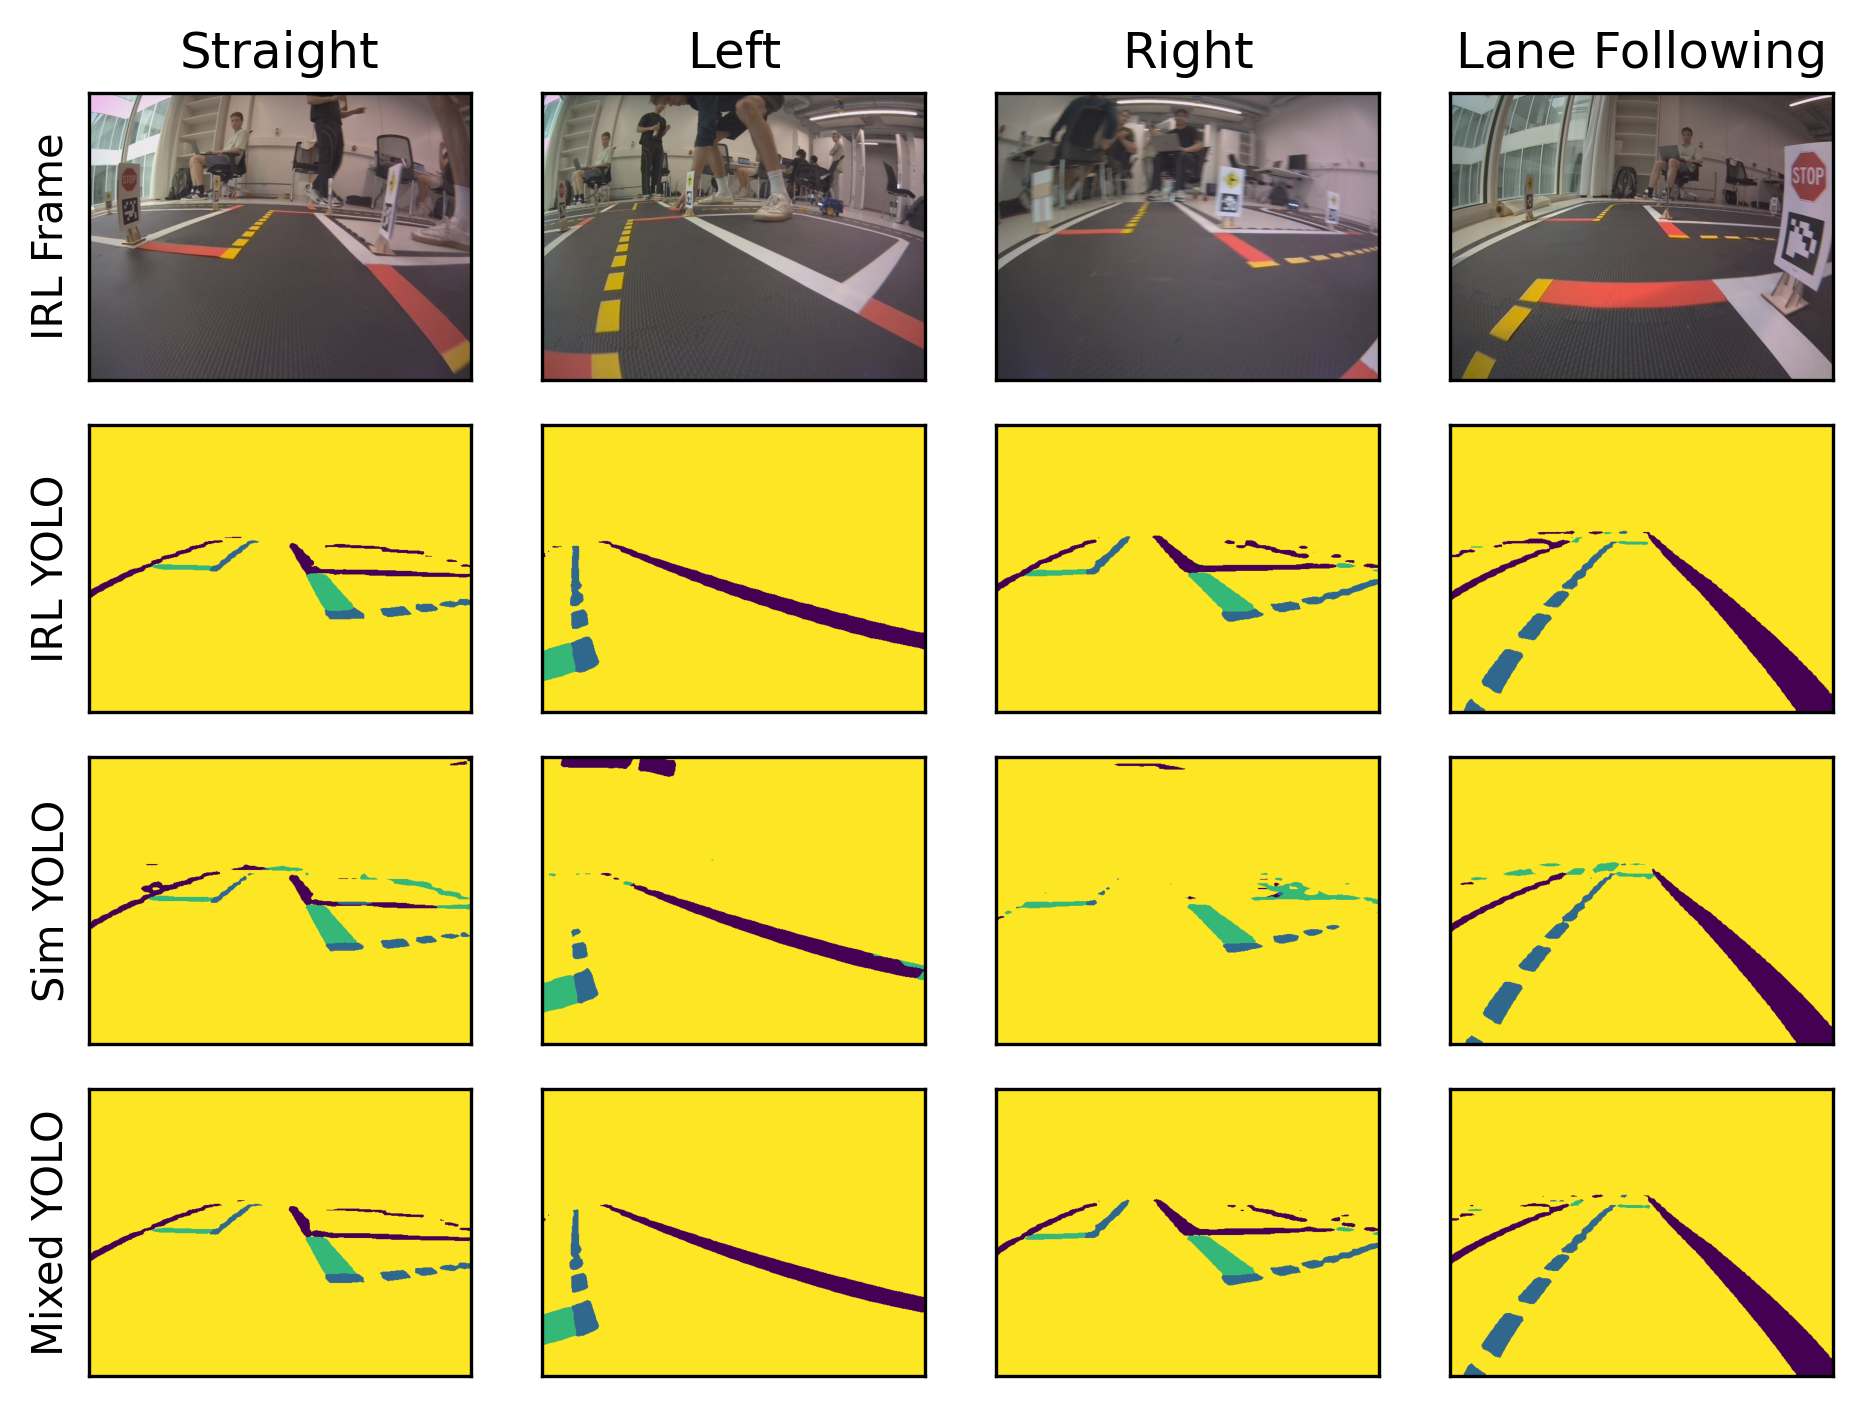
\includegraphics[width=0.8\textwidth]{images/ablation/segmentation/sample_masks_all.png}
    \caption{\textbf{Segmentation Samples:} The figure shows samples from each YOLO26n model trained on either virtual, physical or all data.}
    \label{fig:sample_masks}
\end{figure}

The second ablation we did was regarding the policy network. For all experiments we used the multi-head model depicted in Figure \ref{fig:multipleHeads}. We again trained three variants using virtual data, physical data or both and 
utilized the corresponding YOLO26n model, trained in the first ablation, for each. Subsequently we evaluated their ability to predict the wheel velocities of the physical data. Results are shown in Figure \ref{fig:perf_transfer}

\begin{figure}[H]
    \centering
    \begin{subfigure}[b]{0.8\textwidth}
        \centering
        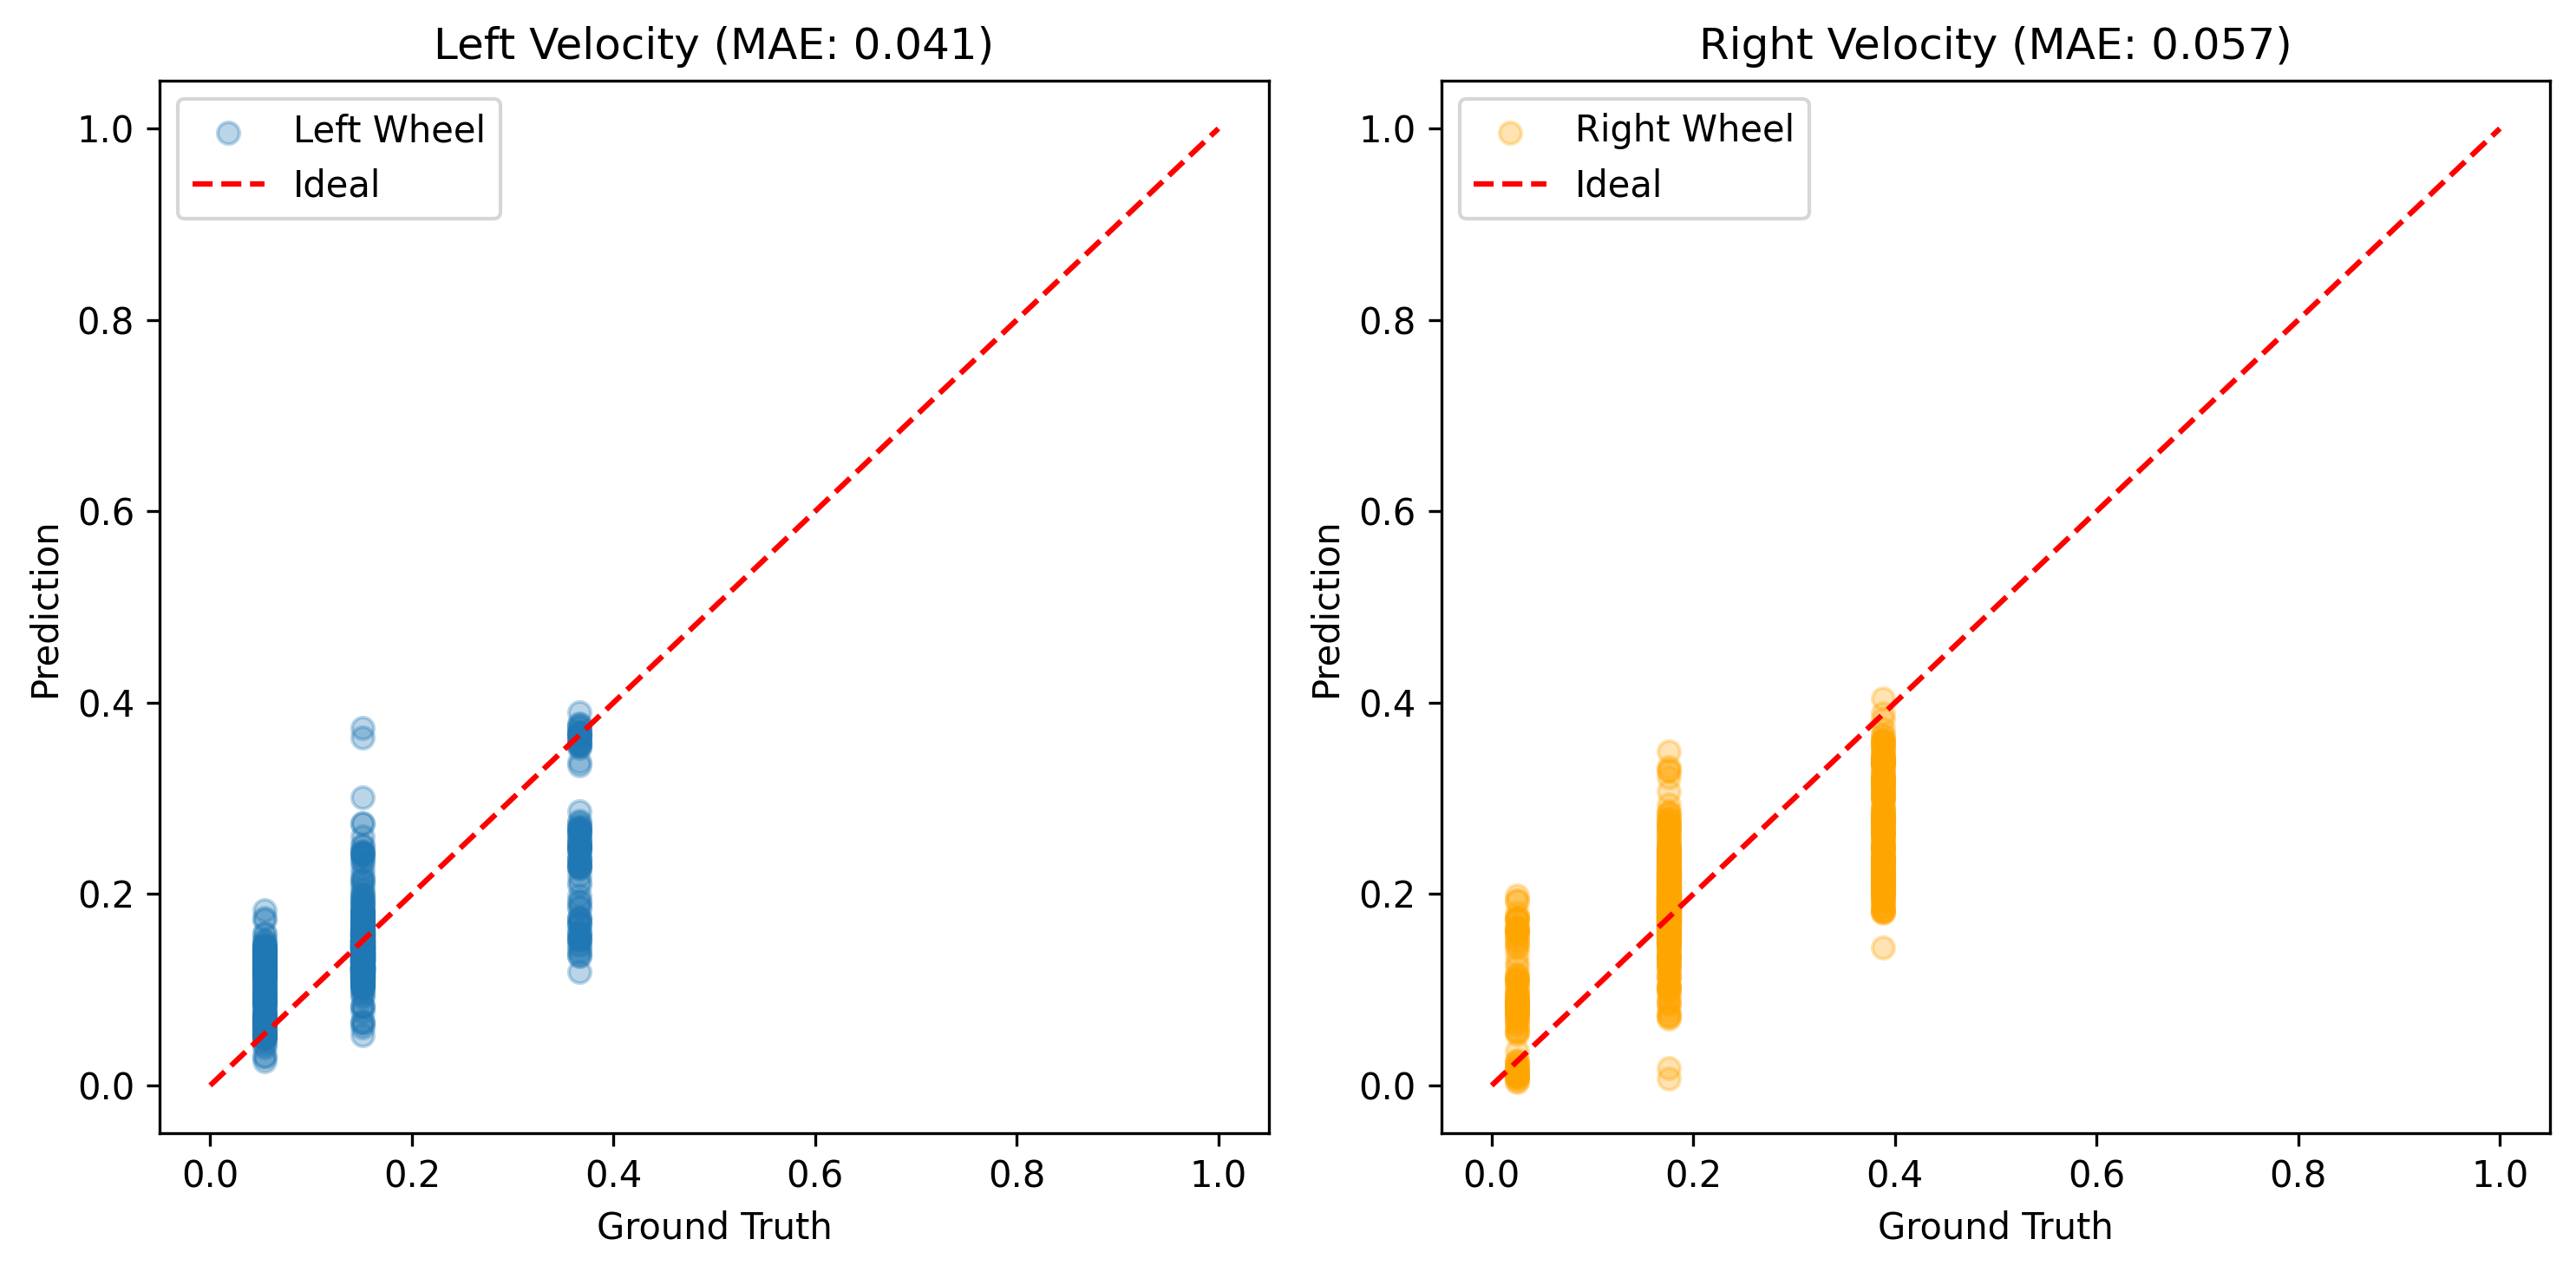
\includegraphics[width=\textwidth]{images/ablation/policy/irl_balanced_velocity_predictions.png}
        \caption{IRL2IRL}
    \end{subfigure}
    
    \begin{subfigure}[b]{0.8\textwidth}
        \centering
        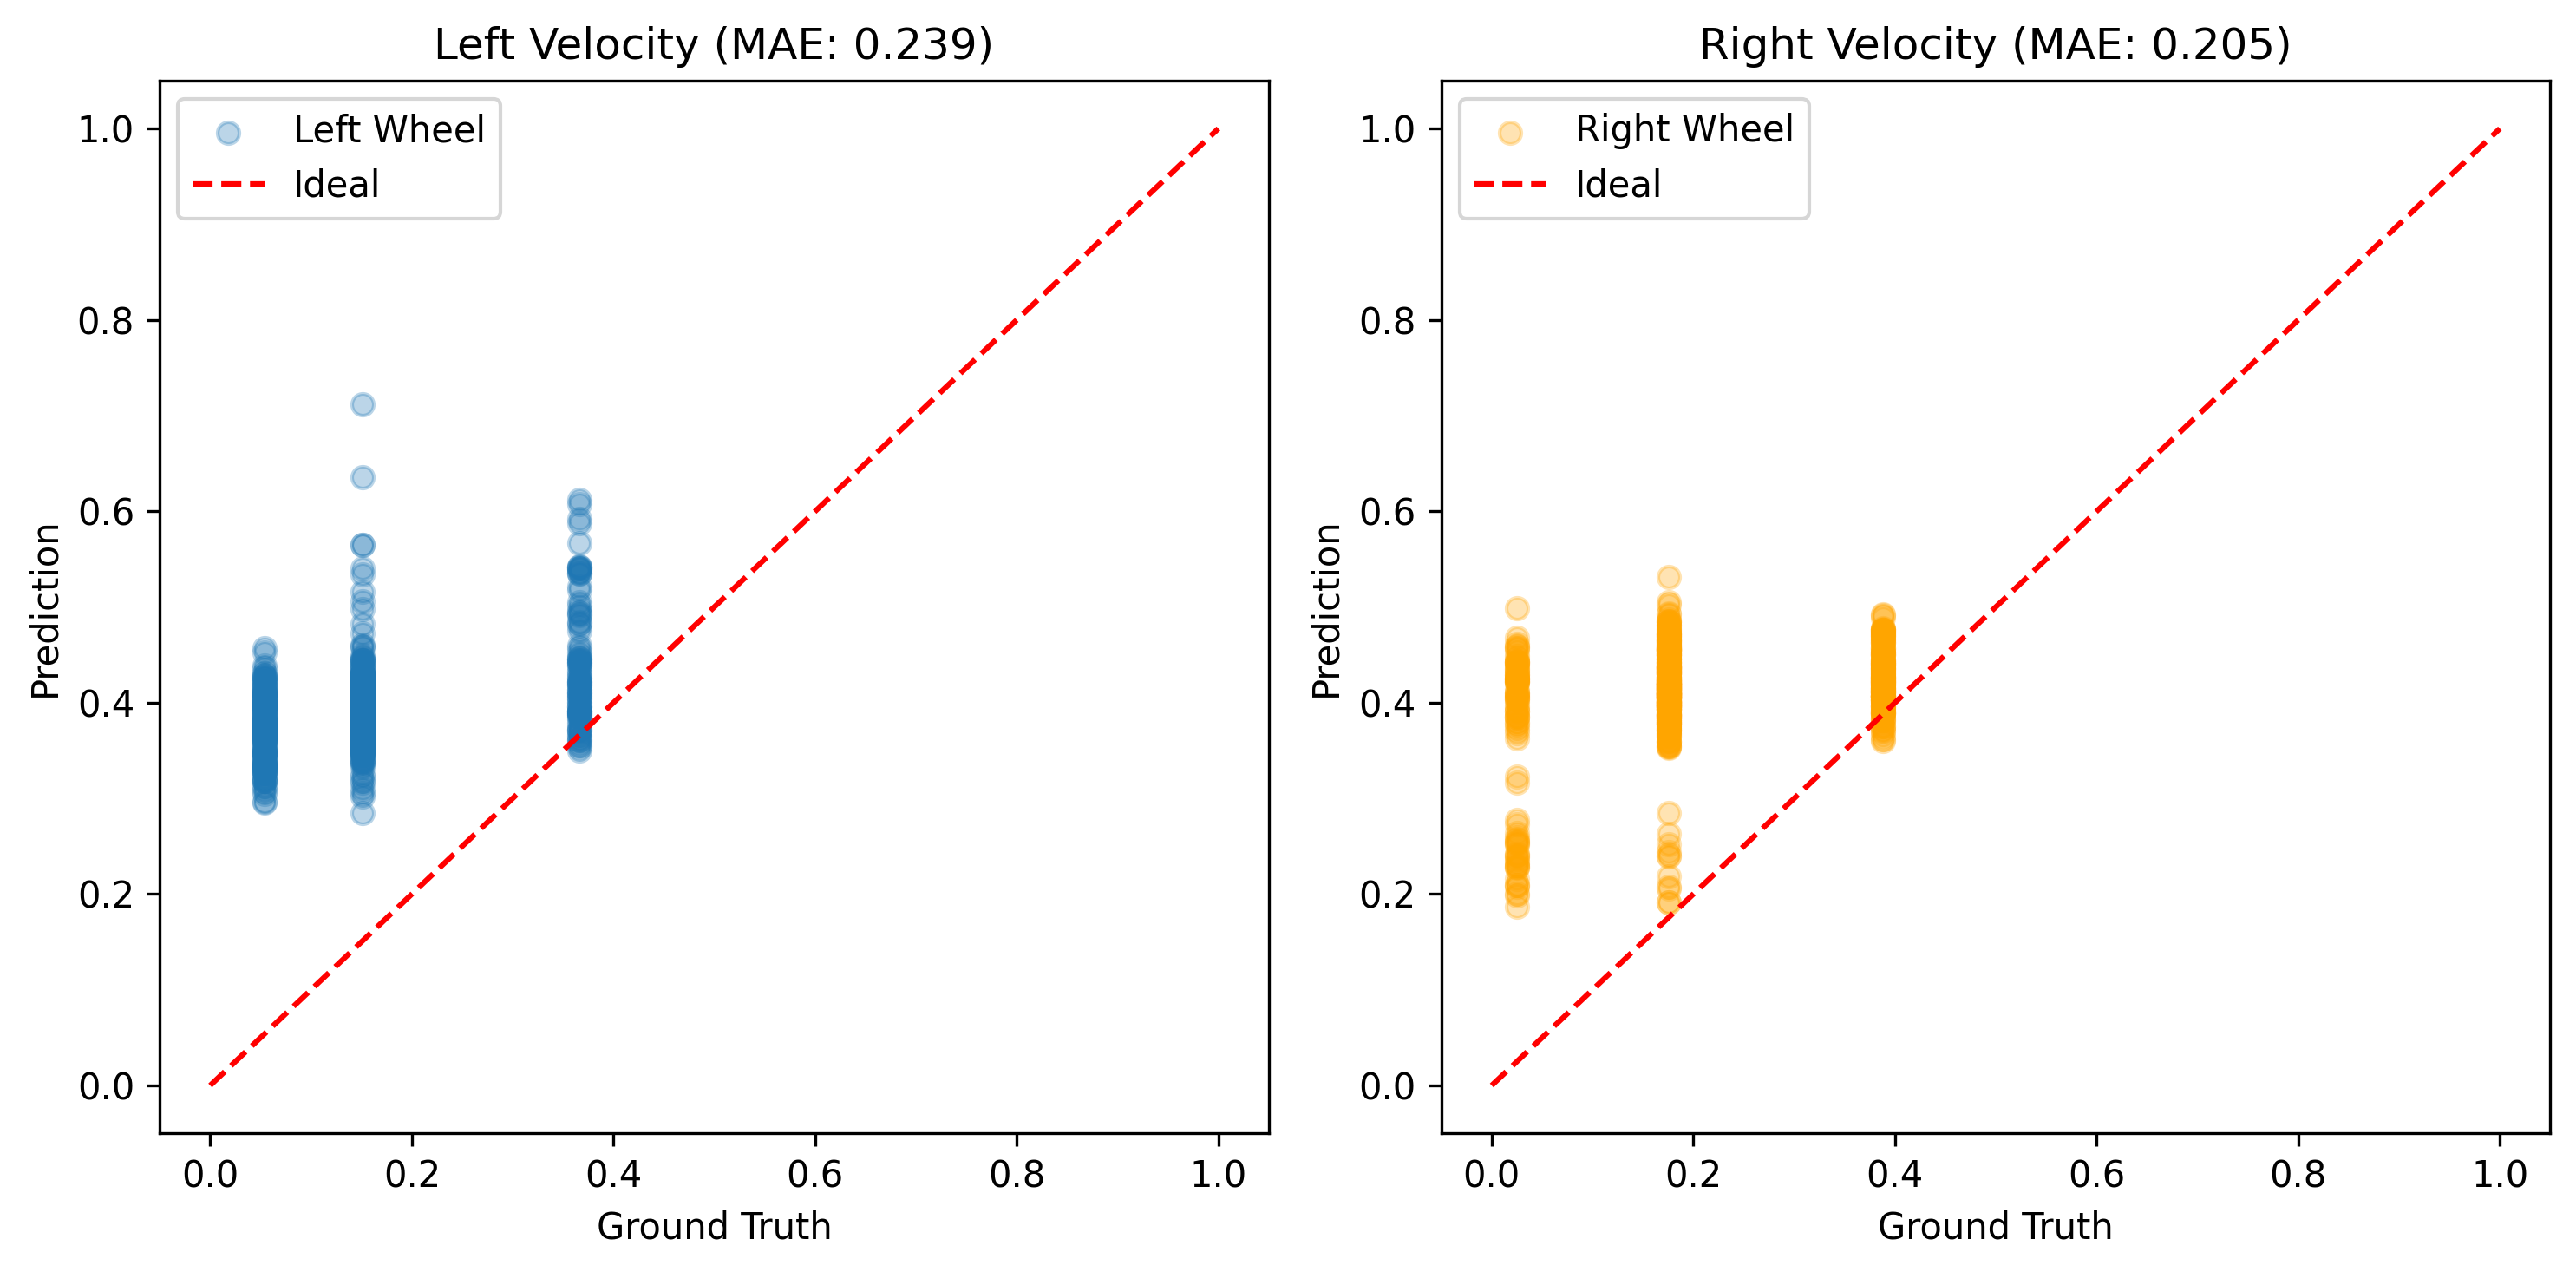
\includegraphics[width=\textwidth]{images/ablation/policy/sim_balanced_velocity_predictions_sim2irl.png}
        \caption{Sim2IRL}
    \end{subfigure}
    
    \begin{subfigure}[b]{0.8\textwidth}
        \centering
        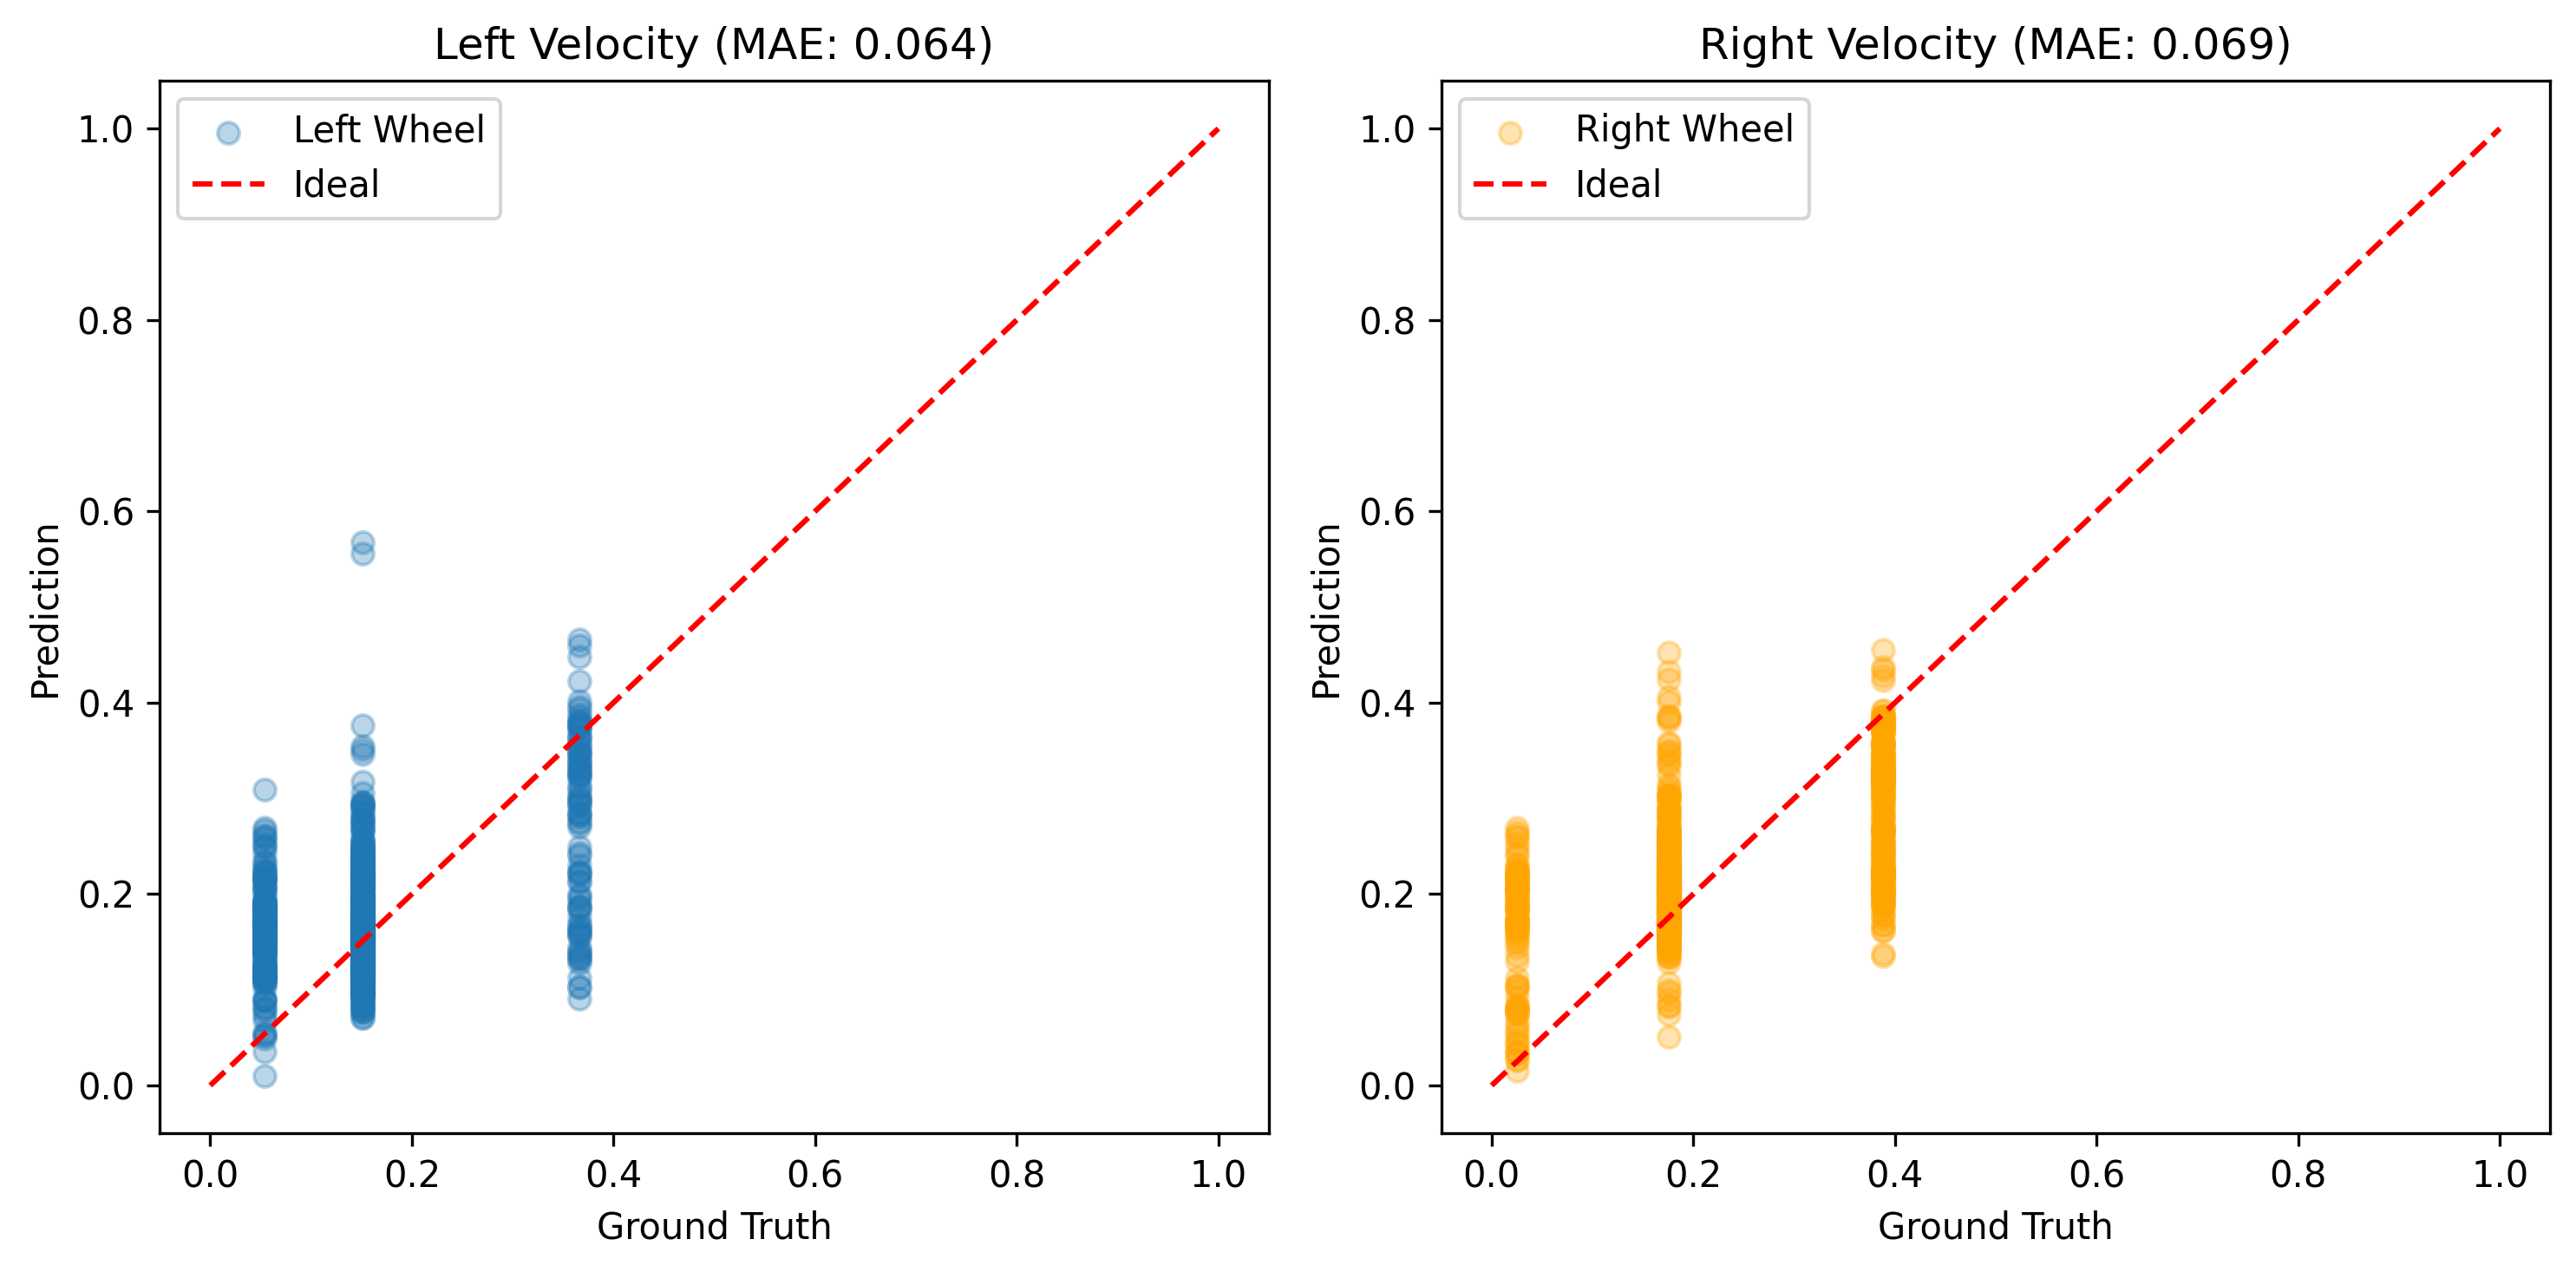
\includegraphics[width=\textwidth]{images/ablation/policy/mixed_balanced_velocity_predictions_mixed2irl.png}
        \caption{Mixed2IRL}
    \end{subfigure}
    \caption{\textbf{Performance Transfer:} Evaluation across different training policies.}
    \label{fig:perf_transfer}
\end{figure}